% capitulo de implementación
\chapter{Diseño e Implementación}
\section{Arquitectura de la solución}
El siguiente capitulo consta de las bases necesarias para realizar la solución. Esta se compone de 2 elementos principales. 
\begin{itemize}
\item Servidor: Encargado de recodificar (si es necesario) la fuente de audio o video y segmentarla para su distribución.
\item Cliente: Aplicación ejecutada en iOS, encargada de comunicarse al servidor para pedir el flujo de video y entregar información en twitter.
\end{itemize}
% poner figura aqui
La figura \ref{diagramaGral} presenta una idea general del sistema.\\

\begin{figure}[h!]
	\centering
	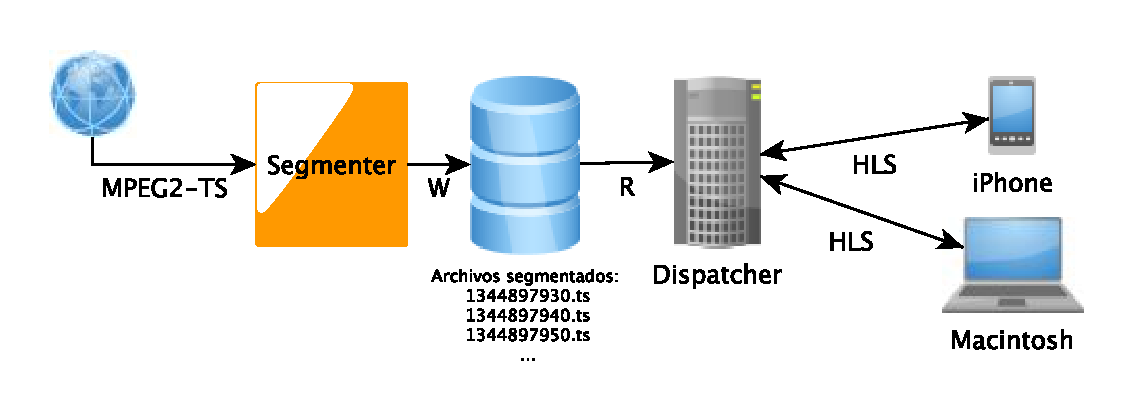
\includegraphics[scale=0.8]{imgs/diagrama_general.eps}
	\caption{Diagrama general de la solución}
	\label{diagramaGral}	
\end{figure}

Respecto a los elementos principales, estos se componen de distintos modulos que serán explicados con más detalle a lo largo del capítulo. Del diagrama se explican de forma general:
\begin{itemize}
\item Segmenter: es una aplicacion que recibe como entrada un flujo de audio y/o video encapsulado en MPEG2-Transport Stream, para luego segmentar el contenido en archivos segmentados de menor duración, estos se guardan en el sistema de archivos del servidor.
\item Dispatcher: Este es un programa dedicado a recibir peticiones de los clientes, para entregar un flujo de video mediante el protocolo HTTP Live Streaming.
\item iPhone y Macintosh: Son los dispositivos clientes controlados por el usuario, en estos se realiza el intercambio de ordenes para recibir el flujo de video que se quiere ver.
\end{itemize}

\subsection{Requerimiento Obligatorio}
% https://developer.apple.com/news/index.php?id=02162010a
	El protocolo utilizado para entregar el contenido audiovisual es HTTP Live Streaming (HLS). Los motivos de esta elección se deben a requerimientos obligatorios designados por Apple para la distribución de contenidos multimedia para su sistema operativo iOS.\\
	
	En un anuncio realizado por Apple en su sitio web destinado a desarrolladores, indica como obligación que la entrega de contenido del tipo audio y/o video con una una duración mayor a 10 minutos debe utilizar el protocolo HTTP Live Streaming ya sea el enlace mediante WiFi o red celular. Además las aplicaciones deben incluir un flujo de datos (stream) de baja calidad con una cadencia de datos no superior a 64 Kilobits/segundo, de manera que estas aplicaciones mantengan fluidez de contenido a pesar de encontrarse en condiciones desfavorables en la red.
	
	En caso de no seguir esta indicación, el desarrollador arriesga que su aplicación no sea admitida en la plataforma principal para la distribución de aplicaciones: iTunes Store.

	Considerando que este trabajo de memoria busca incorporar a los dispositivos iOS como consumidores del contenido multimedia utilizando saltos temporales (TimeShift), se debió diseñar la solucion alrededor de este protocolo.

%en resumen un acercamiento a como funciona la cosa

%\part{Primera parte}
\section{Protocolo HTTP Live Stream}
% https://developer.apple.com/resources/http-streaming/
% http://en.wikipedia.org/wiki/HTTP_Live_Streaming
% http://en.wikipedia.org/wiki/Progressive_download
% http://en.wikipedia.org/wiki/HyperText_Transfer_Protocol

El protocolo HTTP Live Streaming o HLS (abreviado), es un protocolo desarrollado por Apple Inc. para la distribución de multimedia a través de redes de computadores, de manera que el usuario consume el producto a medida que se descarga, es decir de forma continua.\\

Su carácteristica principal es la utilización del protocolo para transferencias de hipertexto, HTTP (hypertext transfer protocol) por sus siglas en inglés. Si bien HTTP se diseño originalmente para la World Wide Web como vía de entrega del texto en formato HTML, este se puede utilzar para distribuir datos de otros formatos codificados para habilitar su distribución.\\

HLS funciona entregando el contenido de forma segmentada al cliente, el cual tiene la responsabilidad de manejar la lógica de cambio de segmentos. Para distribuir el contenido se codifica la fuente de audio y/o video en varios archivos de corta duración, recomendandose entre 5 y 10 segundos, y que pueden o no tener el mismo bitrate. Estos pequeños archivos se ordenan en una lista de reproducción de formato .M3U8 que se entrega al reproductor del cliente. \\
También existe una variante donde la lista de reproducción contiene referencias a otras listas de reproducción con otras variantes de flujos de datos. \\

% http://www.streamingmedia.com/Articles/Editorial/What-Is-.../What-is-HLS-(HTTP-Live-Streaming)-78221.aspx
% In the Apple App Store, if you produce an app that delivers video longer then ten minutes or greater than 5MB of data, you must use  HTTP Live Streaming, and provide at least one stream at 64Kbps or lower bandwidth. Any streaming publisher targeting iOS devices via a website or app should know the basics of HLS and how it’s implemented.
	\subsection{Especificación}
		El protocolo HLS consiste en ordenar la entrega de archivos discretos a través de HTTP.
		El procedimiento general consiste en segmentar el contenido multimedia (audio y/o video) en pequeños archivos de manera que a través de un servidor web regular el cliente pueda descargar y unir los segmentos para verlos de manera continua. Esta forma de entregar el contenido puede ser utilizada para contenido pre-grabado o en vivo, difiriendo levemente en el componente encargado de ordenar los segmentos.\\
		

\clearpage		
\begin{figure}[h!]
	\centering
	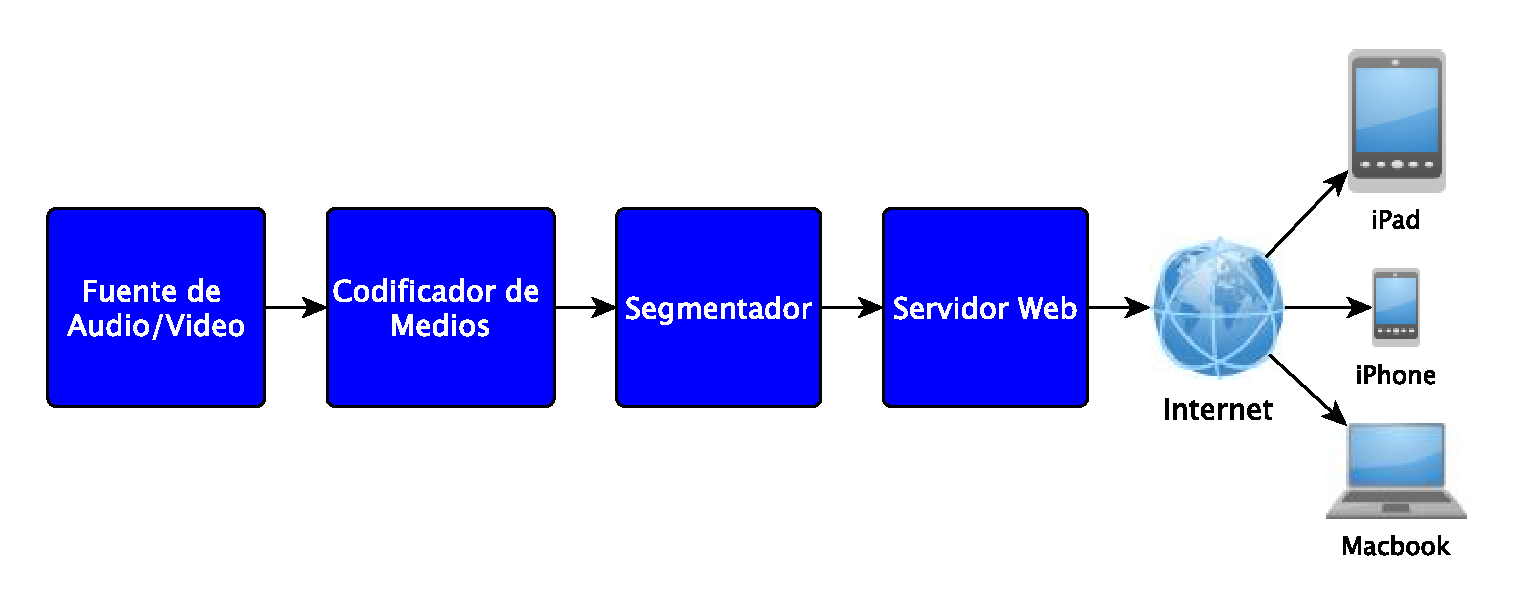
\includegraphics[scale=0.5]{imgs/HLS_diagram_wwdc2010.eps}
	\caption{Flujo de trabajo de HTTP Live Streaming}	
	\label{diagramaHLSwwdc2010}
\end{figure}		
		La figura \ref{diagramaHLSwwdc2010} presenta un ejemplo de distribucion de multimedia a través de HTTP Live Streaming.\\
		
En primera instancia se debe obtener contenido multimedia ya sea en un archivo fijo o flujo de datos, este contenido debe ser codificado para que sea compatible con los dispositivos que corren iOS, generalmente por recomendación de Apple se deben utilizar los codec de video h.264 y de audio AAC (advanced audio coding). El empaquetado de este contenido ya codificado debe ser entregado a una aplicación encargada de segmentarlo en pequeños archivos. \\
	El flujo de transporte a utilizar es MPEG2-TS (MPEG2 Transport Stream), el resultado de la aplicación segmentadora es guardado en el sistema de archivos donde reside el servidor web (o una ubicación accesible) de manera que al recibir requerimientos de stream HLS, este pueda proveer una lista de reproducción en formato M3U8 que mantiene el orden de reproducción de los archivos.\\
	
Tomando en cuenta el funcionamiento del protocolo HLS, para distribuir el contenido multimedia generado en vivo se debe codificar y segmentar inmediatamente para que el servidor web pueda proveerlos. En el caso que el contenido es un gran archivo, la codificación y segmentación se realiza una sola vez.

\subsubsection{Lista de reproducción}
\label{TAG-SECTION}
La lista de reproducción en formato M3U8 es lo entregado al cliente, este puede ser una aplición iOS o el navegador web Safari desarrollado por Apple. Esta lista consiste en enlaces (URL) absolutos o relativos de los segmentos siguiendo el orden del contenido. Además se incluyen comentarios precedidos por el caracter \textbf{\#}, en el caso que un comentario utilice una palabra conocida del protocolo se le denomina entonces como marca (tag).
Las marcas primordiales para una trasmision a través de HLS son las siguientes:

\begin{prop}

\item \#EXTM3U: Corresponde a la primera marca que inicia una lista de reproducción, siempre debe estar al principio.

\item \#EXT-X-TARGETDURATION: Esta marca corresponde a la mayor duración que puede poseer cualquier segmento, es decir los segmentos enumerados en la lista no pasarán del tiempo especificado por esta marca.
Además este valor indica al cliente cada cuanto tiempo debe realizar una petición al servidor web por la lista.
\label{TAG-targetduration}

\item \label{TAG-mediasequence} \#EXT-X-MEDIASEQUENCE: Corresponde a la secuencia o versión de la lista de reproducción segun los segmentos que se incluyen dentro. Este valor se representa por un número entero y debe ser consecuente a los cambios en el contenido, es decir, si se agregan nuevos segmentos el valor de la secuencia debe aumentar, de esta forma el cliente puede saber que el flujo de contenido se está actualizando.


\item \label{TAG-extinfint} \#EXTINF: Esta marca indica la duración del segmento que se encuentra junto a él. Su valor está indicado por un número entero que representa los segundos.\\
\end{prop}

\begin{figure}[h!]
	\centering
	\begin{lstlisting}
	#EXTM3U
	#EXT-X-TARGETDURATION:10
	#EXT-X-MEDIA-SEQUENCE:1
	#EXTINF:10,
	http://media.ejemplo.com/segmento0.ts
	#EXTINF:10,
	http://media.ejemplo.com/segmento1.ts
	#EXTINF:10,
	http://media.ejemplo.com/segmento2.ts
	#EXT-X-ENDLIST
	\end{lstlisting}
	\caption{Lista de reproducción del tipo Video-on-Demand}
	\label{ejemploM3U8}	
\end{figure}			

El ejemplo visto en la figura \ref{ejemploM3U8} destaca una marca extra: \#EXT-X-ENDLIST, la cual indica al cliente que la lista de reproducción está completa y no necesita ser actualizada. Esta marca toma gran importancia al definir un flujo de medios ``en vivo'' ya que al estar ausente el cliente pedirá una nueva versión de la lista de reproducción que incluya nuevos segmentos, el tiempo que indica la actualización depende de la marca \ref{TAG-targetduration} previamente explicada.\\

En el caso de contenido en vivo, la lista de reproducción toma el rol de \textbf{ventana de reproducción}  como la lista se actualiza con nuevos segmentos cada intervalo de \ref{TAG-targetduration} se evita un archivo de gran tamaño al eliminar segmentos ya pasados.

Cabe destacar que la marca \ref{TAG-mediasequence} debe mantener consistencia con los nuevos segmentos, es decir si la lista elimina un segmento pasado y agrega uno nuevo, el numero de secuencia debe aumentar su valor.\\

Para efectos de la solución de este trabajo de memoria el modo de flujo de datos a utilizar con HLS es del tipo ``en vivo''.
\subsubsection{Segmentos}
Los segmentos consisten en video codificado con h.264 y audio en AAC. Apple indica que también es compatible MP3, sin embargo se decidió por AAC debido a su mayor compresión de audio permitiendo así transmitir un mejor sonido a menor ancho de banda. en el anexo XXXX se especifican los codificadores compatibles para la reproducción en iOS, aun así se recomienda utilizar los nombrados anteriormente para mantener compatibilidad para clientes que estén adoptando el protocolo.\\

// TO DO
% El contenedor de los medios es MPEG2-TS según la especificación del protocolo HLS. Las indicaciones de Apple sugieren tener cuidado con el overhead.
		% mostrar figura de playlist, explicacion rapida de como funciona hls
\subsubsection{Borrador IETF}
Apple Inc. es la compañía desarrolladora de este protocolo. Para masificar su uso en dispositivos móviles ha dispuesto un borrador como propuesta para la estandarización del protocolo según la IETF (Internet Engineering Task Force).
Debido a la popularidad de los dispositivos móviles con iOS, empresas importantes en el desarrollo de tecnologias para difusión de medios han adoptado el protocolo HLS como salida de productos dedicados a la codificación y/o transmisión de multimedia. Ejemplos como Adobe Systems con su producto Adobe Flash Media Server, Wowza Media Systems con Wowza Media Server y VideoLan con VLC Media Player demuestran que la documentación realizada por los ingenieros de Apple Inc. Roger Pantos y William May, Jr, deben sentar base para cualquier desarrollo asociado con el protocolo.\\

Para el desarrollo de esta memoria se han implementado aplicaciones y scripts que utilizan las herramientas e instrucciones detalladas en el documento borrador. A lo largo de la investigación los ingenieros desarrolladores incorporaron caracteristicas nuevas que fueron aprovechadas para lograr el cometido de esta memoria.\\

En el anexo YYYY se puede revisar detalladamente el documento completo. En esta sección se describen las marcas utilizadas aparte de las ya descritas en \ref{TAG-SECTION}.

\begin{itemize}
\item \#EXT-X-VERSION: Corresponde a la versión de la lista de reproducción, se utiliza para diferenciar distintos streams con protocolo HLS según las caracteristicas que se van incorporando. Para el trabajo de esta memoria se utiliza la versión 3 del protocolo.

\item \#EXTINF: Si bien ya se ha descrito esta marca en \ref{TAG-extinfint}, a partir de la versión 3 del protocolo HLS, la marca \textbf{EXTINF} permite valores flotantes para mejorar por parte del cliente la exactitud en el seguimiento del tiempo de reproducción. 

\item \#EXT-X-PROGRAM-DATE-TIME: Marca correspondiente a la fecha asociada al primer segmento de datos que aparece en la lista de reproducción. La fecha se especifica utilizando el estandar ISO 8601, opcionalmente se puede incluir zona horaria. Un ejemplo del formato sería:

\begin{lstlisting}
#EXT-X-PROGRAM-DATE-TIME:2011-12-18T14:54:23-04:00
\end{lstlisting}

Correspondiente al día 18 de diciembre de 2011, a las 14:54:23 en la zona horaria GMT-4.

\end{itemize}
		% aqui detallar los mensajes de la playlist utilizados
		%		http://tools.ietf.org/html/draft-pantos-http-live-streaming-08
\subsubsection{Lista de Variantes}
Más allá de la lista de reproducción con segmentos, el protocolo HLS provee de caracteristicas anexas para mejorar la experiencia del usuario.
Una de las caracteristicas a utilizar y que también es requisito para que las aplicaciones con multimedia remota puedan ser aprobada en la App Store es la necesidad de una variante del stream por donde se transmita solamente el audio.\\

Para solucionar este requerimiento y obligación se utiliza una lista de variantes, la cual consiste en una lista de reproducción que incluye en su interior URLs hacia listas de reproducción normales ya explicadas anteriormente, la diferencia cae en que cada lista de reproducción tiene asociado un ancho de banda límite, de manera que el cliente pueda cambiar de stream dentro de la reproducción sin que el usuario note el cambio en la reproducción, exceptuando la calidad del audio o del video.\\

Se utiliza la marca \textbf{\#EXT-X-STREAM-INF} para asociar cada una de las variantes del stream a cierto ancho de banda, además cada una lleva los siguientes atributos:

\begin{itemize}

\item PROGRAM-ID: Corresponde a un valor numérico entero, tiene como fin identificar una presentación en particular dentro de la ventana de transmisión de la lista de reproducción. Una lista de variantes puede contener multiples sublistas con distintos programas de forma que este atributo asocia las distintas variantes para una transmisión en particular, entiendase por show o evento a transmitir. Este atributo puede ser opcional.

\item BANDWIDTH: Este atributo obligatorio representa el valor entero de los bits por segundo, como requisito principal el valor debe ser la cota mayor de la tasa de bits promedio de los segmentos (incluyendo el overhead del contenedor) que aparecen o aparecerán en la lista de reproducción. 

\end{itemize}

El enlace a las sublistas de variantes del stream pueden ser del tipo relativo o absoluto. Como requisito cada variante del stream debe poseer el mismo valor en segundos de Target Duration \ref{TAG-targetduration}.

\begin{figure}[h!]
	\centering
	\begin{lstlisting}
	#EXTM3U
	#EXT-X-STREAM-INF:PROGRAM-ID=1,BANDWIDTH=110000
	varianteA/prog_index.m3u8
	
	#EXT-X-STREAM-INF:PROGRAM-ID=1,BANDWIDTH=200000
	varianteB/prog_index.m3u8

	#EXT-X-STREAM-INF:PROGRAM-ID=1,BANDWIDTH=350000
	varianteC/prog_index.m3u8

	#EXT-X-STREAM-INF:PROGRAM-ID=1,BANDWIDTH=550000
	varianteD/prog_index.m3u8

	#EXT-X-STREAM-INF:PROGRAM-ID=1,BANDWIDTH=900000
	varianteD/prog_index.m3u8

	\end{lstlisting}
	\caption{Lista de variantes para HTTP Live Streaming}
	\label{ejemploVariantPLS}	
\end{figure}	

En la figura \ref{ejemploVariantPLS} se observan tres variantes asociadas al mismo PROGRAM-ID de valor 1. La diferencia entre ellas recae en el ancho de banda límite.\\

Por defecto la primera variante será la utilizada para comenzar la transmisión, y además se utilizará para revisar la calidad del enlace, si la velocidad de descarga de los segmentos da como resultado un mayor ancho de banda, el cliente cambiará a la variante con el mayor valor que pueda cubrir este calculo de ancho de banda.\\

En el caso que exista por distintos motivos una caida en la calidad del enlace, la baja de velocidad de descarga debe ser alertada por el cliente de forma que pueda cambiar la variante en reproducción por otra asociada a un menor ancho de banda. Estos cambios deben ocurrir de manera automatica de modo que al usuario no se le vea afectado el flujo que está consumiendo.\\

Tomando en cuenta este comportamiento, se deben tener consideraciones al armar la lista de variantes según el tipo de enlace que utilizarán sus clientes. Por ejemplo si tiene identificado que sus clientes se conectarán al servidor mediante WiFi es preferible que la lista de variantes tenga como primer elemento la variante de 550000 Kbps y en caso de que sus clientes se conecten al servidor mediante red celular, es preferible presentar como primer variante la de 110000 Kbps.
	De esta forma el cliente reproducirá inmediatamente un stream acorde a su enlace. \\
	
En el ejemplo de la figura \ref{ejemploVariantPLS} a través de red celular el cliente podrá reproducir el contenido rápidamente con velocidades EDGE, y si el enlace lo permite podrá cambiar a una mejor variante. En caso que el cliente se conecte mediante WiFi, cargará el enlace de menor ancho de banda para realizar pruebas e inmediatamente descartarlo por uno de mejor calidad.

% recomendaciones de apple, bitrates y bw



% caracteristicas bacanes de hls, detallar lo que se puede hacer más aun
	\subsection{Herramientas dispuestas por Apple}
	Apple Inc. como desarrollador y promotor de esta tecnología ha dispuesto para los desarrolladores un set de aplicaciones de línea de comandos para la creación de transmisiones con HTTP Live Streaming.
		\subsubsection{MediaFile Segmenter}
Esta aplicación tiene como funcion multiplexar el contenido multimedia del archivo en un flujo de transporte MPEG2 (MPEG2-TS) y dividirlo en una serie de pequeños archivos de aproximadamente la misma duración. La aplicación también crea una lista de reproducción con referencias a los archivos del tipo Video en demanda (VOD).

		\subsubsection{MediaStream Segmenter}
Al igual que MediaFile Segmenter, esta herramienta segmenta el contenido multimedia en varios archivos, sin embargo toma como entrada un flujo de transporte MPEG2 a través de un enlace UDP [dirección:puerto] o también a través de la entrada estandar (stdin). De igual forma que mediafilesegmenter esta aplicación genera una lista de reproducción en formato \textbf{m3u8}.\\

Como recibe de entrada un flujo de datos, permite generar listas de reproducción en vivo, generando segmentos mientras se reciben y actualizando la lista de reproducción con las referencias. Este tipo de flujo de medios es recomendable para difusión contínua, permitiendo además eliminar los segmentos que ya expiraron en la ventana de transmisión.

		\subsubsection{Variant Playlist Creator}
		Esta aplicación se utiliza en conjunto con MediaFile Segmenter para crear una lista de variantes a partir de multiples streams del tipo VOD. Esto se realiza indicando la opcion en MediaFile Segmenter \textit{--generate-variant-plist} que genera un archivo property list (XML) por cada variante del stream, estos archivos se entregan junto a las listas de reproducción para obtener la lista de variante.
			
		\subsubsection{MediaStream Validator}		
		Esta herramienta simula una sesión HLS y verifica que las listas de variantes y reproducción junto a los segmentos cumplen la especificación HTTP Live Streaming. Si se encuentra algún problema en las pruebas de reproducción, se entrega un informe para diagnostico.
		
	\subsection{Ejemplo de transmisión}

Con las herramientas provistas por Apple, se procedió a realizar una transmisión en vivo de prueba, codificando una pelicula ya comprimida en audio AAC y video h.264, los codificadores especificados como compatibles con iOS. Para generar un Stream de video UDP se utilizó la aplicación \textbf{VLC.app} de VideoLan, la cual permite la encapsulación del contenido en MPEG2-TS y su difusión a la misma máquina por UDP utilizando la dirección por defecto \textbf{udp://localhost:1234}. Para realizar esta transimisión se utiliza el \textit{asistente de emisión/transcodificación}.\\

\begin{figure}[h!]
	\centering
	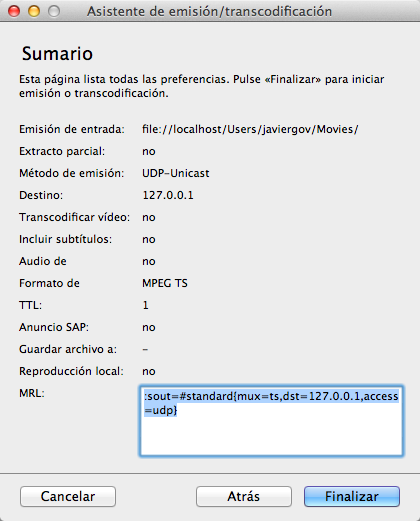
\includegraphics[scale=0.5]{imgs/vlc_transmission.png}
	\caption{Ajustes de la aplicación VLC.app para transmisión de película a través de UDP.}
	\label{vlc_transmission}	
\end{figure}


Considerando las herramientas y el escenario del contenido, la más indicada para transmitir a través de HLS es MediaStream Segmenter ya que puede tomar como entrada el flujo de datos emitidos por UDP y luego entregar su salida a un servidor web Apache que provea a través de internet. De esta forma clientes del tipo iPhone, iPad o Macintosh pueden acceder al contenido multimedia.\\

En la figura \ref{vlc_transmission} se puede observar que la emisión se ha realizado a una ip en específico utilizando el flujo de transporte MPEG2-TS. Este stream se entrega al \textbf{mediastreamsegmenter} con los siguientes parámetros en la línea de comandos.

 \begin{lstlisting}
	mediastreamsegmenter -s 7 -t 11 -D -i ejemplo.m3u8 
	-f ~/Sites/hlsexample 127.0.0.1:1234
\end{lstlisting}

Estos parámetros indican a mediastreamsegmenter que para el ejemplo se genere una lista de reproducción con una ventana de transmisión de \textbf{7} segmentos (\textbf{-s}), los cuales tienen \textbf{11} segundos de duración (\textbf{-t}), además se le indica que los segmentos ya caducados deben ser eliminados (\textbf{-D}). \\

La lista de reproducción lleva el nombre \textit{ejemplo.m3u8} (\textbf{-i}) y los archivos resultantes se deben guardar en el directorio con ruta \textit{$\sim$/Sites/hlsexample} (\textbf{-f}). Por ultimo se indica que la emisión UDP se halla en la dirección ip y puerto: \textit{127.0.0.1:1234}.\\

El resultado de esto es un stream HLS al cual se puede acceder mediante un servidor web como por ejemplo Apache. En caso de este ejemplo los archivos se ubican en el subdirectorio \textit{hlsexample} del directorio asignado a Apache del usuario, para acceder al stream se utilizó un player HTML5 en el archivo \textit{index.html} ubicado junto al resto.

 \begin{lstlisting}
	<html>
	<head></head>
	<body>
		<video src="ejemplo.m3u8" controls 
		autoplay height="360" width="640">
		</video>
	</body>
</html>\end{lstlisting}

Nótese que la fuente al video es la lista de reproducción generada por \textbf{mediastreamsegmenter}, la cual se encuentra en constante actualización mientras la transmisión se lleva a cabo.\\

Ya con el servidor web funcionando, la carga de esta página web permitirá la reproducción del stream en vivo mientras el navegador web sea compatible con el protocolo HTTP Live Streaming utilizando el player HTML5. En la actualidad los únicos navegadores compatibles son Safari y Mobile Safari, desarrollados por Apple.\\
\begin{figure}[h!]
	\centering
	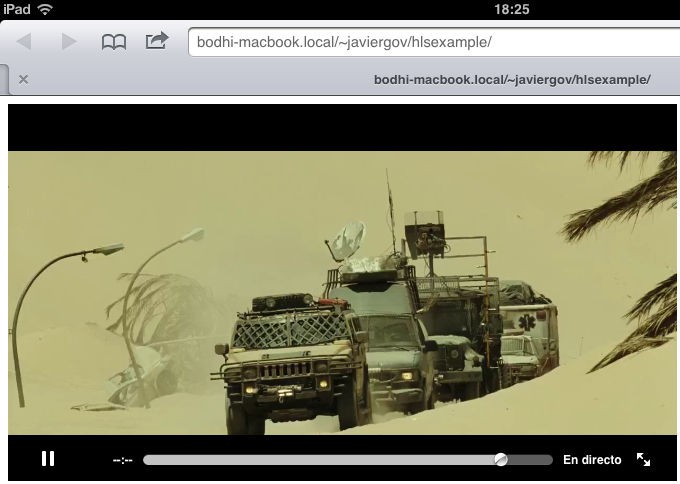
\includegraphics[scale=0.6]{imgs/ipad-hlsexample.png}
	\caption{Captura de pantalla de Mobile Safari en iPad}
	\label{ipad-hlsexample}	
\end{figure}

En la figura \ref{ipad-hlsexample} se puede observar que la reproducción del stream puede ser llevada a cabo por un dispositivo iOS accediendo a la página web creada.\\








	
%	explicar como se probó con resident evil y motorstorm
%	con variantes VOD y live
	
\section{Reproducción y Control de Stream de Video}

%	explicar resumido la estructura como se conecta el server y el cliente, con un  diagrama
	Esta memoria busca entregar control al usuario de la linea temporal de un flujo de contenidos en vivo. Para realizar esto se ideó un sistema que intercambia marcas de tiempo entre el cliente y el servidor, de manera que el cliente pueda definir desde qué punto el servidor debe crear una lista de reproducción en vivo. \\
	
	Para entregar esta información se utilizó como métodos de entrada parámetros en la url que el cliente utiliza para conectarse. Además se puede mejorar la experiencia del usuario indicando al servidor el tipo de enlace que el cliente posee, es decir WiFi o red celular, y expandiendo aun más con un parámetro para definir el canal que se quiere ver, todo desde la misma aplicación.
	
	\subsection{Servidor HTTP}
	El servidor consiste en dos módulos: segmenter y dispatcher, este último depende de los archivos guardados por el segmentador, a su vez el segmentador recibe los datos a través de una emisión UDP o por la entrada estandar \textbf{stdin}.
		\subsubsection{Obtención del Stream}
%		la recepcion de un stream RTMP, codificacion con vlc o ffmpeg y generar un archivo o stream udp
El contenido puede ser obtenido de distintos tipos de fuentes pero este debe cumplir con la especificación de HTTP Live Streaming, es decir entregar al segmentador un flujo de datos codificados con perfiles compatibles con iOS y encapsulados en MPEG2-TS.
		\subsubsection{Sementación del Video}
		% el segmenter que corta su entrada en pedacitos de 10 seg, ademas guarda el tiempo inicial y el final de lo guardado, además se sacarán las fotitos.

El segmentador utilizado fue desarrollado en la empresa AltaVoz S.A. interesada en el proyecto, los motivos de este desarrollo fueron debido a que las herramientas dispuestas por Apple funcionan sólamente en versiones recientes del sistema operativo Mac OS X. Al ver esta limitante la empresa se encarga de desarrollar un segmentador que se comporte de forma similar al \textbf{mediastreamsegmenter}, cortando el stream de entreada en pequeños archivos de cierta duración.\\

 La gran diferencia recalca en el almacenamiento de los archivos resultantes, estos se guardan sin ser eliminados para mantener un gran registro de las transmisiones, el nombre de cada segmento corresponde a la fecha y hora de la recepción de la emisión en formato Unix time (POSIX time) y con extensión \textbf{.ts}. Para mantener orden en el sistema de archivos los segmentos se guardan en subdirectorios por cada hora de contenido, el nombre de estos subdirectorios también llevan Unix time para su catalogación.\\

Una última caracteristica especial del segmentador es marcar el segmento más antiguo y el más reciente en dos archivos \textbf{\textit{start.txt}} y \textbf{\textit{last.txt}} respectivamente, de forma que el cliente pueda representar gráficamente al usuario la disponibilidad de contenido en el stream.
		
		\subsubsection{Emisor de la lista de reproducción}
%		dispatcher que recibe epoch, el tipo (canal) y el bwPARAMETER del tipo de enlace Wifi o cellular		
El \textit{Playlist Dispatcher} consiste en un script \textbf{php} disponible en Internet gracias a un servidor web que trabaje con un módulo PHP, el script \textit{playlist dispatcher} debe recibir parámetros del cliente a través de la cadena de consulta (\textit{query string}) de la dirección URL. Los parámetros son los siguientes:

\begin{itemize}
	\item \textbf{t}: Corresponde a la marca de tiempo que el cliente quiere recibir, esta debe ser indicada con el formato Unix Time (POSIX time).
	\item \textbf{s}: Este parámetro indica al script el cual contenido entregar a través del stream, analogamente se puede considerar como el parámetro para definir cual canal de televisión el usuario quiere ver. El valor corresponde a una cadena de caracteres (\textit{string}).
	\item \textbf{c}: Este último parámetro corresponde al tipo de conexión con la cual el cliente está conectado a Internet, pueden ser dos valores, 1 para red celular y 0 para WiFi. Este parámetro se utiliza para optimizar la lista de variantes que entrega el script.
\end{itemize}
		
Con estos parámetros el script stream es capaz de generar una lista de variantes que referencia a otro script
		
	\subsection{Cliente iOS}
		descripcion general.
		como se conecta al server, reachability, entrega a avplayer
		\subsubsection{Reproducción con AV Framework}
		avplayer, playeritem, asset tracks		
		\subsubsection{Recopilación de datos del Stream}
		kvo, notificaciones, periodic observers, la fecha y que se hace con ella
		
	\subsection{Intercambio de información entre componentes}
	conexión, envio de epoch, recepcion de m3u8, start y last txt	
	
\clearpage
\section{Interfaz Gráfica}
	\subsection{Apple Design Guidelines}
	las guias de diseño y recomendaciones de apple
	\subsection{Componentes de UIKit}
		\subsubsection{UIDatePicker}
		foto, como se usa, el hack para horizontal
		\subsubsection{UIButton}
		play pausa, ibactions
		\subsubsection{...etc}
		volumen, slider de view controller tipo facebook, etc
\clearpage
\section{Integración Redes Sociales}
	diagrama de como funciona el posteo y recepcion de twitts
	\subsection{Twitter}
		\subsubsection{API Twitter}
		las llamadas de twitter que se utilizarán
		\subsubsection{Sharekit vs. Twitter Framework}
		el porqué se utilizó sharekit en vez de twitter framework, el argumento de las apps de twitter
		\subsubsection{Post en Twitter}
		como postear en twitter desde la app, action sheet
		\subsubsection{Seguimiento de Hashtag}
		las llamadas de url para el cliente de twitter
		\subsubsection{Extracción de información de un Tweet}
		como se parseó el json con los twitts y saber si eran sstream
	\subsection{Bit.ly}
		desmenuzar el enlace de bitly
		\subsubsection{API Bit.ly}
		las llamadas de la api que se utilizaron
		\subsubsection{Expansión de atajo bit.ly}
		como se expande un url de bitly y se usa en la app
		\subsubsection{Seguimiento de un Hipervínculo}		
		como se monitorean los twitts por bitly y se puede usar pa marketing, saber que es lo popular etc		

\clearpage
\section{Registro en iOS}
	\subsection{Schemes}
	explicar que son los schemes
	\subsection{Redireccionamiento via Web}
	explicar breve como funcionará la carga del scheme sstream, en web y mobile
		\subsubsection{PHP Script}
		explicar brevemente el script php 
		\subsubsection{Respuestas según User Agent}
		describir los casos según user agents
		
		